%%%%%%%%%%%%%%%%%%%%%%%%%%%%%%%%%%%%%%%%%
% Beamer Presentation
% LaTeX Template
% Version 1.0 (10/11/12)
%
% This template has been downloaded from:
% http://www.LaTeXTemplates.com
%
% License:
% CC BY-NC-SA 3.0 (http://creativecommons.org/licenses/by-nc-sa/3.0/)
%
%%%%%%%%%%%%%%%%%%%%%%%%%%%%%%%%%%%%%%%%%

%----------------------------------------------------------------------------------------
%    PACKAGES AND THEMES
%----------------------------------------------------------------------------------------

\documentclass{beamer}

\usepackage[utf8]{inputenc}
\usepackage[T1]{fontenc}
\usepackage{graphicx}
\usepackage{listings}

\mode<presentation> {

% The Beamer class comes with a number of default slide themes
% which change the colors and layouts of slides. Below this is a list
% of all the themes, uncomment each in turn to see what they look like.

%\usetheme{default}
%\usetheme{AnnArbor}
%\usetheme{Antibes}
%\usetheme{Bergen}
%\usetheme{Berkeley}
%\usetheme{Berlin}
%\usetheme{Boadilla}
%\usetheme{CambridgeUS}
%\usetheme{Copenhagen}
%\usetheme{Darmstadt}
%\usetheme{Dresden}
%\usetheme{Frankfurt}
%\usetheme{Goettingen}
%\usetheme{Hannover}
%\usetheme{Ilmenau}
%\usetheme{JuanLesPins}
%\usetheme{Luebeck}
\usetheme{Madrid}
%\usetheme{Malmoe}
%\usetheme{Marburg}
%\usetheme{Montpellier}
%\usetheme{PaloAlto}
%\usetheme{Pittsburgh}
%\usetheme{Rochester}
%\usetheme{Singapore}
%\usetheme{Szeged}
%\usetheme{Warsaw}

% As well as themes, the Beamer class has a number of color themes
% for any slide theme. Uncomment each of these in turn to see how it
% changes the colors of your current slide theme.

%\usecolortheme{albatross}
%\usecolortheme{beaver}
%\usecolortheme{beetle}
%\usecolortheme{crane}
%\usecolortheme{dolphin}
%\usecolortheme{dove}
%\usecolortheme{fly}
%\usecolortheme{lily}
%\usecolortheme{orchid}
%\usecolortheme{rose}
%\usecolortheme{seagull}
\usecolortheme{seahorse}
%\usecolortheme{whale}
%\usecolortheme{wolverine}

%\setbeamertemplate{footline} % To remove the footer line in all slides uncomment this line
%\setbeamertemplate{footline}[page number] % To replace the footer line in all slides with a simple slide count uncomment this line

%\setbeamertemplate{navigation symbols}{} % To remove the navigation symbols from the bottom of all slides uncomment this line
}

\usepackage{graphicx} % Allows including images
\usepackage{booktabs} % Allows the use of \toprule, \midrule and \bottomrule in tables

%----------------------------------------------------------------------------------------
%    TITLE PAGE
%----------------------------------------------------------------------------------------

\title[Linux Container APIs]{Container management APIs} % The short title appears at the bottom of every slide, the full title is only on the title page

\author{Serge Hallyn} % Your name
\institute[Canonical] % Your institution as it will appear on the bottom of every slide, may be shorthand to save space
{
Canonical, Ltd \\ % Your institution for the title page
\medskip
\textit{serge.hallyn@ubuntu.com} % Your email address
}
\date{\today} % Date, can be changed to a custom date

\begin{document}

\lstset{language=sh}

\begin{frame}
\titlepage % Print the title page as the first slide
\end{frame}

\begin{frame}
\begin{figure}
  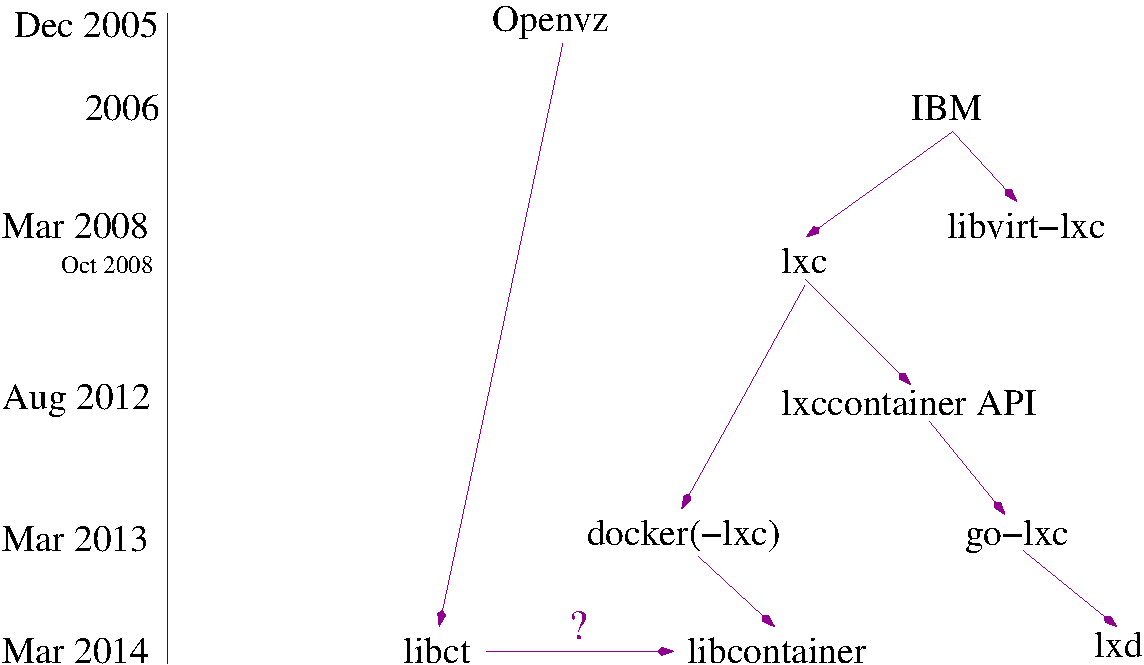
\includegraphics[width=\textwidth]{timeline.pdf}
\end{figure}
\end{frame}

\begin{frame}
\frametitle{Regular Usage: Overview}
\begin{itemize}
\item Let's first go over the basics:
  \begin{itemize}
  \item Download an image
  \item Run a command in a container
  \item query images and containers
  \item Publish the new image
  \end{itemize}
\item Demos
  \begin{itemize}
  \item docker
  \item lxd
  \item lxc
  \item libct
  \end{itemize}
\end{itemize}
\end{frame}

\begin{frame}
\frametitle{Digging Deeper}
\begin{itemize}
\item Getting familiar with the commands is important
\item Docker and LXD have REST APIs
  \begin{itemize}
  \item Docker
    \begin{itemize}
    \item 
    \end{itemize}
  \item LXD
    \begin{itemize}
    \item 
    \end{itemize}
  \end{itemize}
\end{itemize}
\end{frame}

\begin{frame}
\frametitle{Runc}
\begin{itemize}
\item A new way to run OpenContainers format containers
\item (Usable from other languages - which go pkgs are not)
\item Requires
  \begin{itemize}
  \item untarred rootfs
  \item config.json: mounts (brief), user, env, capabilities, arch
  \item runtime.json: mounts(details), devices, security, hooks, more
  \end{itemize}
\end{itemize}
\end{frame}

\begin{frame}
\frametitle{Building new tools}
\begin{itemize}
\item libcontainer
  \begin{itemize}
  \item 
  \end{itemize}
\item libct
  \begin{itemize}
  \item 
  \end{itemize}
\item LXD/LXC
  \begin{itemize}
  \item 
  \end{itemize}
\end{itemize}
\end{frame}


%------------------------------------------------

\end{document} 
